% グラフを作成するコマンド
\newcommand{\myfigure}[2]{
    \begin{figure}[htbp]
        \centering
        \includegraphics[width=17.7cm]{#1}
        \caption{#2}
        \label{fig:#2}
    \end{figure}
}

% \newcommand{\reffigure}[1]{図\ref{fig:#1}(\pageref{fig:#1}ページ)} % ページ数も載せる場合
\newcommand{\reffigure}[1]{図\ref{fig:#1}} % ページ数を載せない場合





\section{実験}





改造したMiniSatと実装した遺伝アルゴリズムを用いて実際に証明の作成を行なった。
主な実験として
\begin{enumerate}
    \item 遺伝アルゴリズムのパラメータを調整して、短い証明を作りやすくするための実験
    \item 調整を行なった遺伝アルゴリズムがどれぐらいの効果あるかをみる実験
    \item 最先端のソルバーと比べてどれぐらい短い証明が作れているのかをみる実験
\end{enumerate}
の3種類の実験をおこなった。
実験のために用いる問題は、SATソルバの性能を測る大会SAT compの2016年のAgileトラックにおいて、
ベンチマークとして使われた問題を使用した。
遺伝アルゴリズムの出力結果を表すグラフは横軸に世代、縦軸にMiniSat比で見た証明の長さをおき各染色体の証明の長さを見た。
すべて縦軸の範囲は0から1までに限定している。
また事前の実験として、特定のタイミングで重みの書き換えを行うのではなく1つの変数を選択した場合の証明を作成する実験と、
遺伝アルゴリズムを使わずに8回の介入をタイミングを変えた場合の証明の違いを確認する実験を行なった。





\setcounter{subsection}{-1} % 事前実験の小節番号が0になるように





\subsection{事前実験}

% 1変数選択による介入
1つ目の事前実験として1変数介入による証明作成を行なったが、
すぐに元の変数選択に戻ってしまうためほとんど同じ証明が作成された。
本実験においては介入の際に変数の重みを書き換えているが、
重みを変更するのではなく変数を1つ指定してそのタイミングでは指定した変数を選んだ際に、
どれぐらい短い証明ができるかという実験を行なっている。
結論としてこの時にできる証明は介入をしなかった元の証明とほとんど同じ長さの証明が作成された。
このようなことが起きる原因を探るために介入直後のMiniSatの挙動について調べた。
MiniSatがどの変数を選択しているかを介入をした場合としていな場合で確認したところ、
介入をした時点においては確かに指定した変数を選んでいるが、次の変数選択においては介入をしなかった場合に選ばれる変数が選ばれ、
そこからはほとんど同じ変数選択になっていた。
これは1つ変数を選択したところで変数の重みは書き変わっていないため、
次の変数選択からは介入をしなかった場合の変数選択と同じ流れになってしまうことが考えられる。
変数の重みは矛盾が発生した場合に変数の重みが書き換わるので、
唯一介入直後に矛盾が起きた場合にのみ通常の変数選択とは少し異なる変数選択になる
そのため1つの介入でより広い範囲の変数選択に影響を与えられるように本実験では重みへの介入を行う方法を採用している。
なお、1つ変数を選択する場合の選び方として、ランダムに変数を選ぶやり方や、
1から10番目に重みが大きい変数を実際に選んだ場合における証明の長さが一番短かった変数を選択するといった選び方などを行なった。

\todo{(2つ目の内容はあとで)}

2つ目の事前実験としてタイミングを変えながら8回の介入を行い証明を作成した。
結論として後半の変数選択に集中して介入すると短い証明ができにくいという結果が得られたが
その他の場合においてはそれぞれにあまり違いがなかったため、
遺伝アルゴリズムの初期集団を作成する際には各染色体の介入のタイミングはランダムに選ぶようにした。

\myfigure{figures/Experiment0/1.png}{タイミングずらしつつ8回介入}

\reffigure{タイミングずらしつつ8回介入}はそれぞれ8回の介入タイミングを固定して介入を500回行った時の
証明の長さの分布を表したものである。
問題は後のパラメータ調整で用いられる問題と同じ問題を使用した。
この時の各介入におけるシード値はランダムに設定している。
介入のタイミングは2つ目の方法をのぞいて元の変数選択数$n(={約}40000{回})$を基準としており、それぞれ左から
\begin{enumerate}
    \item 介入が等間隔になるように$n/8, 2n/8, ..., 8n/8$回目で介入
    \item 5000回ごとに介入
    \item 序盤で集中して介入するために$n/24, 2n/24, ... , 8n/24$回目で介入
    \item 中盤で集中して介入するために$9n/24, 10n/24, ... , 16n/24$回目で介入
    \item 終盤で集中して介入するために$17n/24, 18n/24, ... , 24n/24$回目で介入
    \item 前の介入ほど短い間隔で介入するために後ろの介入になるにつれて間隔が3/2倍ずつ長くなるように介入(最後の介入は$n$回目)
    \item 前の介入ほど長い間隔で介入するために後ろの介入になるにつれて間隔が2/3倍ずつ短くなるように介入(最後の介入は$n$回目)
\end{enumerate}
という風な介入を表している。

グラフを見るとわかるように4,5,7番目の介入方法における分布の幅は他の介入方法よりも小さくなっており、
短い証明を作りにくくなっていることがわかる。
そのため、後ろのタイミングで多く介入するような介入ほど短い証明を作りにくくなっていることがわかる。
その他の介入方法については分布の差や最小値の差を見るとあまり違いがないのがわかる。
以上のことから介入のタイミングはランダムで設定することで実験を行っている。






\subsection{パラメータ調整}



まず最初の実験として遺伝アルゴリズムのパラメータ調整を行う実験を行なった。
問題を1つ固定し、遺伝アルゴリズムがより効果的に作用するようにパラメータの調整をしている。
調整を行なったのは以下の4つで、実験によってそれぞれ
\begin{itemize}
    \item 初期集団を作成する際の各染色体の介入数はランダムに選択
    \item 集団のサイズを200
    \item 世代数は30世代
    \item 突然変異を行う際は元の介入の1割を追加・削除
\end{itemize}
といった調整がなされている。
問題はあまり時間がかからない数秒で解けるような問題
\footnote{MiniSatで1.7秒、drat-trimで2.9秒ほどかかる問題で、証明の長さが約25000、変数選択数が約40000回の問題}
を採用した。

% 通常の6000倍ぐらいの実行時間
% 遺伝アルゴリズムはパラメータ調整がが必要



% 1.初期状態
\subsubsection{初期状態}

最初に現在の遺伝アルゴリズムを実行しその効果を見た。
集団サイズは5で20世代まで作成、初期集団の各染色体の介入の回数は10回で固定し、
突然変異の際の介入の追加・削除数は1としている。

\myfigure{figures/Experiment1/1.png}{初期パラメータにおける全染色体の証明長}

\reffigure{初期パラメータにおける全染色体の証明長}を見るとわかるように、13世代目で大きく良い個体が作成されているだけで、
それ以外の世代では大きく良い個体が作成されているような箇所はない。
また多様性の観点で見ると12世代目まではほとんどの個体が90\%付近に集中しており、
多様性があまりないようにが感じられる(初期世代のみ90\%から135\%の範囲に点が散らばっていた)。
加えて最終世代の各個体の介入タイミングがどのように分布しているかを見たところ、
どの個体もほとんど同じタイミングでの介入になっておりほぼ収束してしまっていることが考えられる。
そのため次に集団の多様性を上げるような調整を行なった。
なお、ここでの一番短い証明はもとの証明の60\%ほどの証明であった。



% 2.集団サイズと世代数を増加
\subsubsection{集団サイズと世代数を増加}

次の実験では集団のサイズと世代数を増やす調整を行なった。
ここでは集団のサイズを20、世代数を25にして増やした上で遺伝アルゴリズムを実行した。
この変更によって集団の多様性が増え、より短い証明が作成されることを期待している。

\myfigure{figures/Experiment1/2.png}{集団サイズと世代を増加}

結果として初期の結果よりも短い証明を作成することができた。
\reffigure{集団サイズと世代を増加}を見ると、2世代目で良い個体を2つも作ることができているが、
そこから数世代はほんの少し良い個体ができているだけで、
5世代目以降ではほとんどの個体が50\%弱のあたりに集まる形になってしまいすぐに収束してしまっている。
集団の解が収束してしまっている原因として、介入の回数が少なすぎることが考えられる。
ここまでの実験において初期介入数として設定した10という数はとりあえずで設定したものであり、
どの介入数が適切であるかはわかっていないため、次の実験として介入数をランダムにする変更を行なった。
集団のサイズと世代数についてはこの変更によって初期状態より良い個体を作成できているので、
変更後の状態で次の実験を行う。



% 3.集団サイズと世代数を増加
\subsubsection{介入の回数をランダムに}

次の実験として、介入の回数をランダムにして遺伝アルゴリズムを実行した。
ここでのランダムは最初の世代を作成する際に各染色体が持つ介入の回数を、
1回から何もせず解かせた場合の変数選択数(この問題においては約40000回)の間でランダムに決めるという意味である。
先ほどの実験を通して集団数は20、世代数は25世代に変更している。

\myfigure{figures/Experiment1/3.png}{初期の介入回数をランダムに}

実験の結果として、\reffigure{初期の介入回数をランダムに}を見るとわかるように、
後半の世代においても個体の評価値(証明の短さ)に幅が生まれており前の実験よりも収束しにくくなっていることがわかる。
学習が進んでいるかという点で見ると、良い染色体を更新できてはいるがいささか無駄が多いようにも感じる。
図を見ると2,8,17世代目では最良の個体を更新できているが、それ以外の世代の多くは集団が上の方に移動してしまっており、
せっかく作った良い個体を活かしきれていないように感じられる。
特に5世代においては全ての個体の評価値が1以上になってしまっている。
この対策として集団をサイズをさらに増やすことを考えている。
集団のサイズを増やすことで良い個体を作る機会が増え、さらに親として選択する際に良い個体を選択する機会が増えるため、
良い個体をさらに活かすことができるのではと考えた。
なお、以降の実験では介入の回数はランダムにするように変更した。

\paragraph{適切な介入回数について}

今回介入回数をランダムにしていたのは適切な介入回数がわからなかったためであり、
とりあえずでランダムに設定していた。
学習が進んだ後の介入の回数を見ることで適切な介入回数の方針が得られるのではないかと考え、
それを見るために作成したグラフが\reffigure{介入回数の遷移}である。

\myfigure{figures/Experiment1/3-1.png}{介入回数の遷移}

グラフを見ると最後の方の世代では全ての個体の介入の回数が15000回付近に集中していることがわかる。
このことからも作成した遺伝アルゴリズムは何らかの学習が進んでいることがわかる。
そのため、介入の回数が15000ぐらいが短い証明を作りやすいのではないかと考え、
初期の介入の回数の範囲を10000から20000でランダムというかたちに変更して実験を行なった。

\myfigure{figures/Experiment1/3-2.png}{介入回数を10000以上20000以下で始める}

結論としてこの変更は良い変更とはいえなかった。
範囲を変えた場合における実験では変える前の実験に比べると良い個体が作れていないという結果になっており、
\reffigure{介入回数を10000以上20000以下で始める}を見るとわかるように変更前よりも多くの個体が100\%以上の証明を作成している。
加えて世代が進むにつれてほんの少し良い個体ができることもあり学習はほんの少し進んでいるが、
変更前に比べると良い個体はできておらず、ほとんど学習が進んでいないともいえる。
そのため以降の実験では初期介入回数の範囲を狭めることはせずに、もとのランダムのかたちで遺伝アルゴリズムを実行している。



% 4.集団サイズと世代の変更
\subsubsection{集団サイズと世代の変更}
次の実験として介入をランダムにした状態における適切な集団のサイズと世代数を探す実験を行なった。
今回は遺伝アルゴリズム1回の実行において評価回数を定めておき、その中で集団のサイズと世代数を変更させた。
このときの評価回数は、今回の研究において他の実験に影響を与えすぎない、1回の実行時間で許容できる最大の評価回数にしている。
遺伝アルゴリズムの実行時間の中で大部分を占めるのは染色体を評価する部分であり、
1つの染色体につき1回の評価を行うため、いくつの染色体を作成するかでおおよその実行時間を予測することができる。
この染色体を作る回数は集団のサイズ*世代数に等しい。
つまり同じ評価回数のもとでは集団のサイズと世代数はトレードオフの関係にある。
今回は1回の実行で許容できる最大の評価回数を6000で固定しその回数の元で集団のサイズと世代数を変更した。
3種類の実験を行いそれぞれ
\begin{itemize}
    \item 集団サイズ100 * 世代数60
    \item 集団サイズ150 * 世代数40
    \item 集団サイズ200 * 世代数30
\end{itemize}
の設定の元で遺伝アルゴリズムを実行しその中で一番適切だと思われる設定を採用した。
なお各遺伝アルゴリズムの実行時間は9時間から13時間ほどであった。

実験を通して、集団のサイズは200、世代数は60で設定して以降の実験を行うことに決定した。
図\ref{fig:集団サイズ100、世代数60}から\ref{fig:集団サイズ200、世代数30}(\pageref{fig:集団サイズ100、世代数60}ページ)は
それぞれの設定の元での遺伝アルゴリズムの実行結果をグラフにしたものである。
全体として、集団のサイズが小さい場合には早く収束してしまっていた。

\begin{figure}[h]
    \centering
    \begin{minipage}{0.43\columnwidth}
        \centering
        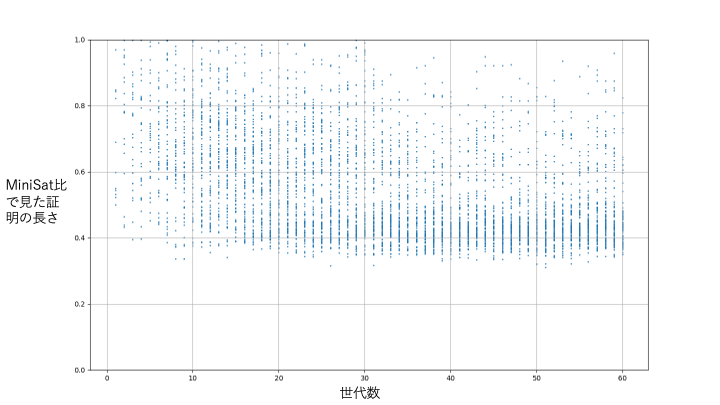
\includegraphics[width=1.2\columnwidth]{figures/Experiment1/4-1.png}
        \caption{集団サイズ100、世代数60}
        \label{fig:集団サイズ100、世代数60}
    \end{minipage}
    \hspace{5mm}
    \begin{minipage}{0.43\columnwidth}
        \centering
        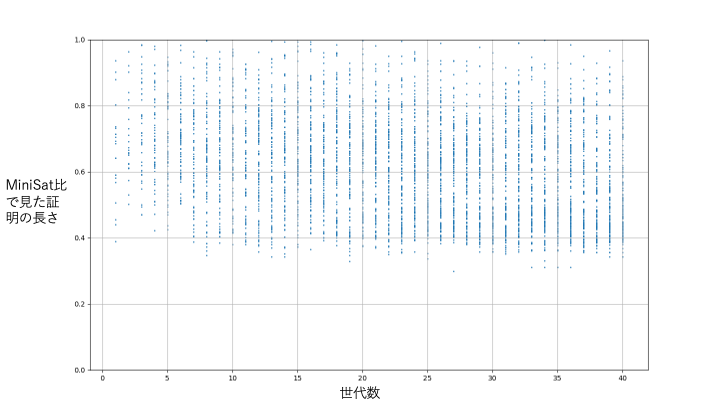
\includegraphics[width=1.2\columnwidth]{figures/Experiment1/4-2.png}
        \caption{集団サイズ150、世代数40}
        \label{fig:集団サイズ150、世代数40}
    \end{minipage}
  
    \vspace{3mm}
    
    \begin{minipage}{0.43\columnwidth}
        \centering
        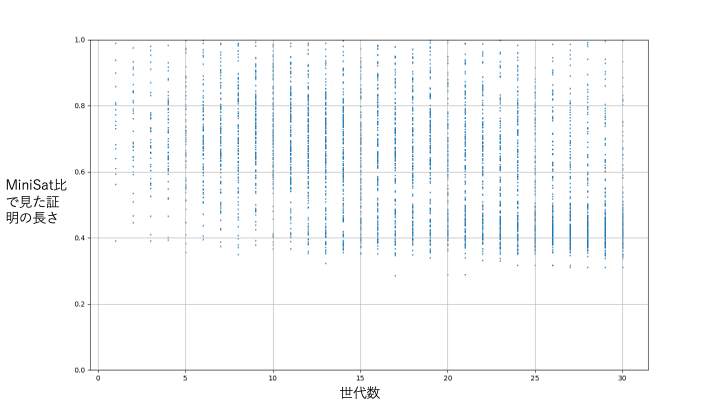
\includegraphics[width=1.2\columnwidth]{figures/Experiment1/4-3.png}
        \caption{集団サイズ200、世代数30}
        \label{fig:集団サイズ200、世代数30}
    \end{minipage}
    \hspace{5mm}
    \begin{minipage}{0.43\columnwidth}
        \centering
        
\includegraphics[width=1.2\columnwidth]{figures/white.png}
    \end{minipage}
    \caption*{評価回数を6000として集団サイズと世代を変更}
\end{figure}

まず図\ref{fig:集団サイズ100、世代数60}を見ると、40世代以降においては多くの点が40\%付近に集中しているのがわかり、
解がほとんど収束しているように見える。
解が収束してしまっている状態での探索は局所解の探索であり、この先で大きく改善された解を見つけるは難しい。
そのため解が収束した状態以降の探索はそれまでの探索に比べると無駄な部分になっており、
できるだけこの部分は排除したい。

これに対して世代数を少なくした図\ref{fig:集団サイズ150、世代数40}のグラフは図\ref{fig:集団サイズ100、世代数60}に比べると
最終世代でもあまり収束していないのが読み取れる。
そのため収束性という点ででみると集団サイズ150、世代数40の方が集団サイズ100、世代数60よりも良い設定であると考えられる。

最後に集団サイズ150、世代数40の設定と集団サイズ200、世代数30の設定を比較したところ、後者の設定の方が学習がうまく進んでいるような印象が感じられた。
実際に前の世代よりも良い個体を作成できた回数を調べたところ前者は約2.3回に1回良い個体を作成できたのに対して、
後者は2回に1回いい個体を作成できていた。
また、最終世代における集団の評価値の幅を見たところ、前者は34\%から154\%の幅に対して、後者は31\%から450\%となっており多様性にも違いがあった。
なお、集団サイズ100、世代数60においては35\%から131\%の間に点が存在した。
以上の結果と考察から以降の実験においては集団サイズを200、世代数を30に設定して遺伝アルゴリズムを実行した。



% 5.突然変異の変更
\subsubsection{突然変異の変更}
最後の変更として突然変異の変更を行なった。
今までは介入を1つ追加または削除する突然変異を使っていたが、介入を元の1割追加もしくは1割削除するという方法の突然変異に変更した。
この変更の理由としては初期の介入の回数が10回からランダムになったためである。
介入の回数がランダムになったため今回の問題においては各染色体が持つ平均介入数は20000回ほどであり、
この場合において介入を1つ追加したり、削除したりしてもほとんど効果がないと考えたためである。
この突然変異の変更を行い最後に初期の状態とどれくらい変わったのかと、ランダムな介入とどれぐらい違うのかを比較した。
ランダムな介入は遺伝アルゴリズムの実行時間とほぼおなじにするために6000回行った。

% 横にランダムと初期状態のベスト置きたい
\myfigure{figures/Experiment1/5.png}{突然変異の変更}

\reffigure{突然変異の変更}は突然変異を変更した後における遺伝アルゴリズムを実行した結果を表したグラフであり、
赤線は初期状態における一番短い個体の証明の長さ、黄色線はランダムに介入をした場合における一番短い個体の証明の長さを表したものである。
図を見るとわかるように調整を行なった最終的な遺伝アルゴリズムは初期状態やランダムな介入よりも短い証明を作れていることがわかる。
今回の実行においては26世代目にできた個体の証明が一番短くもとの証明の29\%ほどの証明であった。
またこの証明は初期状態の証明の45\%ほどの長さであり、ランダムな証明の95\%ほどの長さの証明となった。
なお、ランダムにおける証明ははもとの証明の長さの30\%ほどの長さの証明であった。


% 6.ランダムとの比較 
% \subsubsection{ランダムとの比較}



%  ・実行時間を短縮できないかという目的





\subsection{色々な問題に対して解く}%6ページ



続いての実験として、先ほど設定したパラメータのもとで様々な問題を解き、作成した遺伝アルゴリズムの効果を見た。
最初に前の実験で使用した問題と同じぐらいの難易度の問題やより難しい問題に対して効果を確認した。
その後各問題においてどれぐらい短くなったかを確認した。
また、学習がうまくいっているような問題に対してさらに学習を続けた場合にどのような結果になるかを見た。
全体の結論として全て短い証明を作成することができた。



% 1.同じくらいの難易度の問題を解く
\subsubsection{同じくらいの難易度の問題を解く}

まず最初にパラメータの調整に使用した問題と同じくらいの難易度の問題に対して遺伝アルゴリズムを実行し、
もとの問題と同じぐらい短い証明を作成できるかを見た。
ここでの難易度は問題に対してMiniSatとdrat-trimを実行した時にかかる秒数とした。
パラメータ調整に使用した問題は4.6秒ほどで解ける問題であったため、同じくらいの難易度の問題として数秒で解ける問題を3問使用した。

\myfigure{figures/Experiment2/1.png}{数秒で解ける問題の1例} % 4125

\reffigure{数秒で解ける問題の1例}はその中の1問に対する実行結果である。
なおこの問題はminisat4秒、drat-trim5.6秒ほどかかる問題であった。
図を見るとわかるように遺伝アルゴリズムによってもとの問題よりも短い証明が作れていることがわかる。
一番良い個体は10世代目で作成されており、今回の問題においては元の証明の51\%ほどの証明を作成することができた。
また1世代目よりも良い個体を作成できており、学習が進んでいることがわかる。
しかし10世代目までは学習が進んでいるものの、それ以降においては世代が上下しているだけで学習があまり進んでないことがわかる。



% 2.より難しい問題を解く
\subsubsection{より難しい問題を解く}
続いてより難しい問題に対して遺伝アルゴリズムを実行した。
より難しい問題を解いた理由の1つとしては、難しい問題ほどその解き方に改良の余地があり、
より短い証明を作成することができるのではないかと考えたためである。
秒数としては20秒から100秒ほどの問題に対して遺伝アルゴリズムを使用した。
結論としては一部の問題に対しては前の実験よりも短い証明を作ることができたが、ほとんどの問題においては似たような結果が得られた。
なお問題を解いている途中でほとんどの問題は30世代進めなくても学習が進んでいるかやどれくらい短い証明ができるかの予測ができたので、
一部の問題に対しては10世代までの実行で終了している。

\myfigure{figures/Experiment2/2.png}{難しい問題の1例} % 10118

\reffigure{難しい問題の1例}はその中の1問に対する実行結果である。
グラフを見てわかるようにほんの少し学習が進んでおり、初期の世代より良い個体の生成に成功しているが、
11世代目以降作成してみてもここから大きく学習が進むようなことはないことが感じ取れる。
また、この時の最良の個体の証明はもとの証明の45\%ほどの長さの証明を作成しており、
さきほど1例としてあげた問題とほぼ同じ縮小率であった。
違う点でいうとこちらの問題の方がより個体が下の方によっている点がグラフから読み取れる。



% 3.各問題のベストを見る
\subsubsection{各問題のベストを見る}

これら全ての問題に対して結果的にどれくらい短い証明が作れているのかをグラフを作成して確認した。

\myfigure{figures/Experiment2/3.png}{問題の難易度と遺伝アルゴリズムの効果(赤い点は追加で行なった問題)}

\reffigure{問題の難易度と遺伝アルゴリズムの効果(赤い点は追加で行なった問題)}は横軸に介入前の実行時間、
縦軸に各問題に対して遺伝アルゴリズムを実行した時に作成できた一番短い証明の長さをおいたグラフである。
ここでの実行時間はMiniSatとdrat-trimの実行時間としているが、
MiniSatのみやdrat-trimのみの実行時間としてグラフを作成した場合も似たようなグラフになっていた。
赤い点については後から追加した点であり、後のパラグラフで説明する。

グラフを見るとどの問題に対しても元の証明よりも短い証明を作成できていることがわかる。
また20秒から60秒の問題については10\%以下になるような証明も作成できていた。
なお、作成できた証明の幅について調べたところ、最小だと6\%ほどの証明になり、最大だと85\%ほどの長さの証明であった。

\paragraph{60秒から100秒の問題を追加で解く}
\reffigure{問題の難易度と遺伝アルゴリズムの効果(赤い点は追加で行なった問題)}のグラフを見てみると60秒から100秒における4つの青い点が
40\%から60\%強の範囲に集まっているがわかる。
それより前の20秒から60秒の問題はより広い範囲に点が分布してため、
この点の集まりかたはたまたまであるのか、それとも必ずこのあたりに点が集まってしまうのかが気になった。
そこで60秒から100秒の問題に対して追加で実験を行なった。
\reffigure{問題の難易度と遺伝アルゴリズムの効果(赤い点は追加で行なった問題)}における赤い点は追加で実験を行なった問題の結果を表したものである。
グラフを見るとわかるように赤い点は40\%から60\%強の範囲よりも外側にある場合も多くあり、
この範囲に青い点が集まっていたのは偶然であることがわかる。
なお赤い点を含めた場合は点の範囲は13\%から69\%ほどの範囲まで拡大していた。



% 4.学習が続いている問題を解く
\subsubsection{学習が続いている問題を解く}

前述したようにいくつかの問題については10世代目までで遺伝アルゴリズムの実行を終了していたが、
いくつかの問題については学習が進んでいるような状態を観測することができ、
11世代目以降も同じペースで学習が進んでより短い証明を作成することができるのではないかという疑問が生じた。
そこで学習が進んでいるような問題のいくつかに対して追加でもう10世代集団を作成し、結果を見た。
結論として、追加で行なったどの問題についても同じペースで減り続けることはなくすぐに学習が進まなくなった。

\myfigure{figures/Experiment2/4.png}{学習が進んでいる問題の1例}

\reffigure{学習が進んでいる問題の1例}は実際に実験を行なった問題の中の1つをグラフにしたものである。
赤い線の前半1から10世代目が追加で実験を行う前の結果で、後半11から20世代目が追加で実験を行なった後に得られた結果である。
グラフを見るとわかるように前半世代においては順調に良い個体が増えていっており、
この先追加で世代を作った場合にさらに良い個体が作成されることが期待される。
初期世代と10世代目の最良の個体を比較した時に、初期世代では最良が26\%であったのに対し10世代目では10\%になっているため、
更に実行を続けていけば同じペースで学習が進み数\%ほどの証明が作成されてもおかしくない。
しかし、実際に実行を続けてみたところ同じペースで学習が進むことはなかった。
後半の世代を見てみるとほとんど最良の個体を更新できていないことがわかる。
後半の世代の中で一番最良の個体はもとの10\%の証明の長さなので、前半の世代と比較してみても確かに学習が進んでいない。
実行を追加で続けてみても同じペースで学習が進まないというこの現象は他の問題についても同様に観測された。


\subsection{最先端ソルバとの比較}

最後の実験として今回作成した証明は最先端ソルバが作成する証明とどれくらい違うのかを確認する実験を行なった。
今回は最先端ソルバとしてKissatを使用し、
問題に対してKissatとdra-trimを実行した時に作成される証明を最先端ソルバの証明としている。
そのため6000回MiniSatとdrat-trimを実行する遺伝アルゴリズムとは時間に関して大きな差があるが、
本研究では時間をかけても短い証明を作ることを目標にしているのでこの点は考慮しないものとする。

\myfigure{figures/Experiment3/1.png}{最先端ソルバとの比較}

\reffigure{最先端ソルバとの比較}はそれぞれの問題に対して横軸にKissatが作成した証明の長さ、
縦軸に遺伝アルゴリズムによって作成できた証明の中で1番短い証明の長さをMiniSat比で表したものである。
直線は$y=x$の線であり、この直線の下にある点においては遺伝アルゴリズムがKissatより短い証明を作れたことを表している。
また両軸の範囲は0から1の間に制限しているが、どの問題も全てこの範囲に収まっていた。
グラフを見てみると、前述したように遺伝アルゴリズムによって作成した証明はMiniSatよりも短い証明を作成できていることがわかるが、
Kissatより短くなるような証明ができている問題はほとんどなく、
Kissatに勝てていてもその証明の長さはKissatの証明の長さとほとんど変わらないことがわかる。
今回問題として57問の問題を解いたが、その中でKissatに勝ていたのは8問であった。
また勝てていた問題については、最小でKissatの59\%ほどの証明を作れていたものが1つあったが
それ以外の問題は全てKissatの70から100\%の長さの証明に収まっていた。
また右下の方に点が全くないことからも今回実装した遺伝アルゴリズムによって作成した証明はKissatにまったく勝てていないことがわかる。
この原因についてはいくつか存在するがその1つとしては、
Kissatがすでにほとんど最適な証明を作成しているという可能性である。
つまりどのように時間をかけて証明を作ったとしてもその証明がKissatに勝てないということである。
このような右下に点がないことに対する課題や原因については後のセクションの中で説明を行う。

\subsection{今後のために少し調べたこと}

今後のために少し調べた実験として親選択時の適応度の変更を行なった。
新しい子を生成する際、環境に適応している個体ほど親として選択しやすくすることで、
より評価の高い個体を生成しやすくなる操作を行っている。
これを再現するために個体の評価値からどれだけ環境に適応しているかを表す適応度を計算し、
この適応度を重みとしてランダムに選択することで適応度の高い個体ほど親として選択されやすくするようにしている。
ここまでの遺伝アルゴリズムにおいては評価値である証明の長さの逆数をとることによって、
証明が短い個体ほど親として選択されやすいように実装していた。
この適応度の計算を逆数から逆数の2乗に変更して実験をおこなった。
これによりより短い証明を作成しやすくなることを期待している。
デメリットとして、より親として良い個体をとりやすくなると悪い個体を早く淘汰してしまい、
解が速く収束してしまう恐れがある。

\myfigure{figures/Experiment4/1.png}{適応度の変更(左が変更前、右が変更後)}

\reffigure{適応度の変更(左が変更前、右が変更後)}はある問題について適応度の変更前後での実行結果をグラフにしたもので、
左のグラフが変更前のグラフで右のグラフが変更後を表している
この問題はパラメータ調整で使用した問題とは別の問題となっている。
グラフを見るとわかるように変更前においては4世代目までは最良の個体を更新しており学習が進んでいるが、
5世代目以降は逆に各世代における最良の個体がどんどん悪くなっている。
一方で変更後においてはより長い世代まで学習が進んでいるように思われる。
また6世代目においては変更前の最良の個体よりも大きく良い個体の生成に成功している。
変更前ではもとの51\%の証明が一番短かったのに対し変更後では34\%の証明を生成しており、
変更前の66\%の長さの証明となっている。


